\let\negmedspace\undefined
\let\negthickspace\undefined
\documentclass[journal,12pt,onecolumn]{IEEEtran}
\usepackage{cite}
\usepackage{amsmath,amssymb,amsfonts,amsthm}
\usepackage{algorithmic}
\usepackage{graphicx}
\graphicspath{{./figs/}}
\usepackage{textcomp}
\usepackage{xcolor}
\usepackage{txfonts}
\usepackage{listings}
\usepackage{enumitem}
\usepackage{mathtools}
\usepackage{gensymb}
\usepackage{comment}
\usepackage{caption}
\usepackage[breaklinks=true]{hyperref}
\usepackage{tkz-euclide} 
\usepackage{listings}
\usepackage{gvv}                                        
%\def\inputGnumericTable{}                                 
\usepackage[latin1]{inputenc}     
\usepackage{xparse}
\usepackage{color}                                            
\usepackage{array}
\usepackage{longtable}                                       
\usepackage{calc}                                             
\usepackage{multirow}
\usepackage{multicol}
\usepackage{hhline}                                           
\usepackage{ifthen}                                           
\usepackage{lscape}
\usepackage{tabularx}
\usepackage{array}
\usepackage{float}
\usepackage{parskip}
\newtheorem{theorem}{Theorem}[section]
\newtheorem{problem}{Problem}
\newtheorem{proposition}{Proposition}[section]
\newtheorem{lemma}{Lemma}[section]
\newtheorem{corollary}[theorem]{Corollary}
\newtheorem{example}{Example}[section]
\newtheorem{definition}[problem]{Definition}
\newcommand{\BEQA}{\begin{eqnarray}}
\newcommand{\EEQA}{\end{eqnarray}}
\newcommand{\define}{\stackrel{\triangle}{=}}
\theoremstyle{remark}
\newtheorem{rem}{Remark}

\begin{document}
\title{2.8.32}
\author{EE25BTECH11045 - P.Navya Priya}
\maketitle
\renewcommand{\thefigure}{\theenumi}
\renewcommand{\thetable}{\theenumi}

\textbf{Question:}

Ayush starts walking from his house to office. Instead of going to the office directly, he goes to a bank first, from there to his daughter school and then reaches the office. What is the extra distance travelled by Ayush in reaching his office? If the house is situated at $(2,4)$, bank at $(5,8)$, school at $(13,14)$ and office at $(13,26)$ and coordinates are in km.

\vspace{0.5cm}
\textbf{Solution:}

Let us solve the given equation theoretically and then verify the solution computationally.\\[5pt]
Let's assume the coordinates as

\begin{table}[H]
\centering
\renewcommand{\arraystretch}{1}
\begin{tabular}{|m{1cm}|m{1cm}|}
\hline
  $\vec{H}$   &  $\myvec{2\\4}$ \\ \hline 
  $\vec{B}$   &  $\myvec{5\\8}$ \\ \hline
  $\vec{S}$   &  $\myvec{13\\14}$ \\ \hline
  $\vec{O}$   &  $\myvec{13\\26}$ \\ \hline
\end{tabular}
\end{table}

To calculate the extra ditsance travelled by Ayush, let d$_1$ be the distance from his home to office
\begin{align}
    \text{d}_1\,&=\,||\vec{O}-\vec{H}||\\[4pt]
    \,&=\,\sqrt{\myvec{\vec{O-H}}^\top\myvec{\vec{O-H}}}\\[4pt]
    \,&=\,\sqrt{605}\,\text{km}\brak{\approx 24.59}
\end{align}

Let d$_2$ be the actual distance travelled by Ayush,
\begin{align}
    \text{d}_2\,&=\,||\vec{B}-\vec{H}||\,+\,||\vec{S}-\vec{B}||\,+\,||\vec{O}-\vec{S}||\\[4pt]
    \,&=\,\sqrt{\myvec{\vec{B-H}}^\top\myvec{\vec{B-H}}}\,+\,\sqrt{\myvec{\vec{S-B}}^\top\myvec{\vec{S-B}}}\,+\,\sqrt{\myvec{\vec{O-S}}^\top\myvec{\vec{O-S}}}\\[4pt]
     \,&=\,27\text{km}
\end{align}

The extra distance travelled is,
\begin{align}
    \text{d}_2\,-\,\text{d}_1\,&=\,27-24.59\\[4pt]
    \,&=\,2.41\,\brak{\approx2.4\text{km}}
\end{align}

\newpage
From the graph, theoretical solution matches with the computational solution.

\begin{figure}[H]
\centering
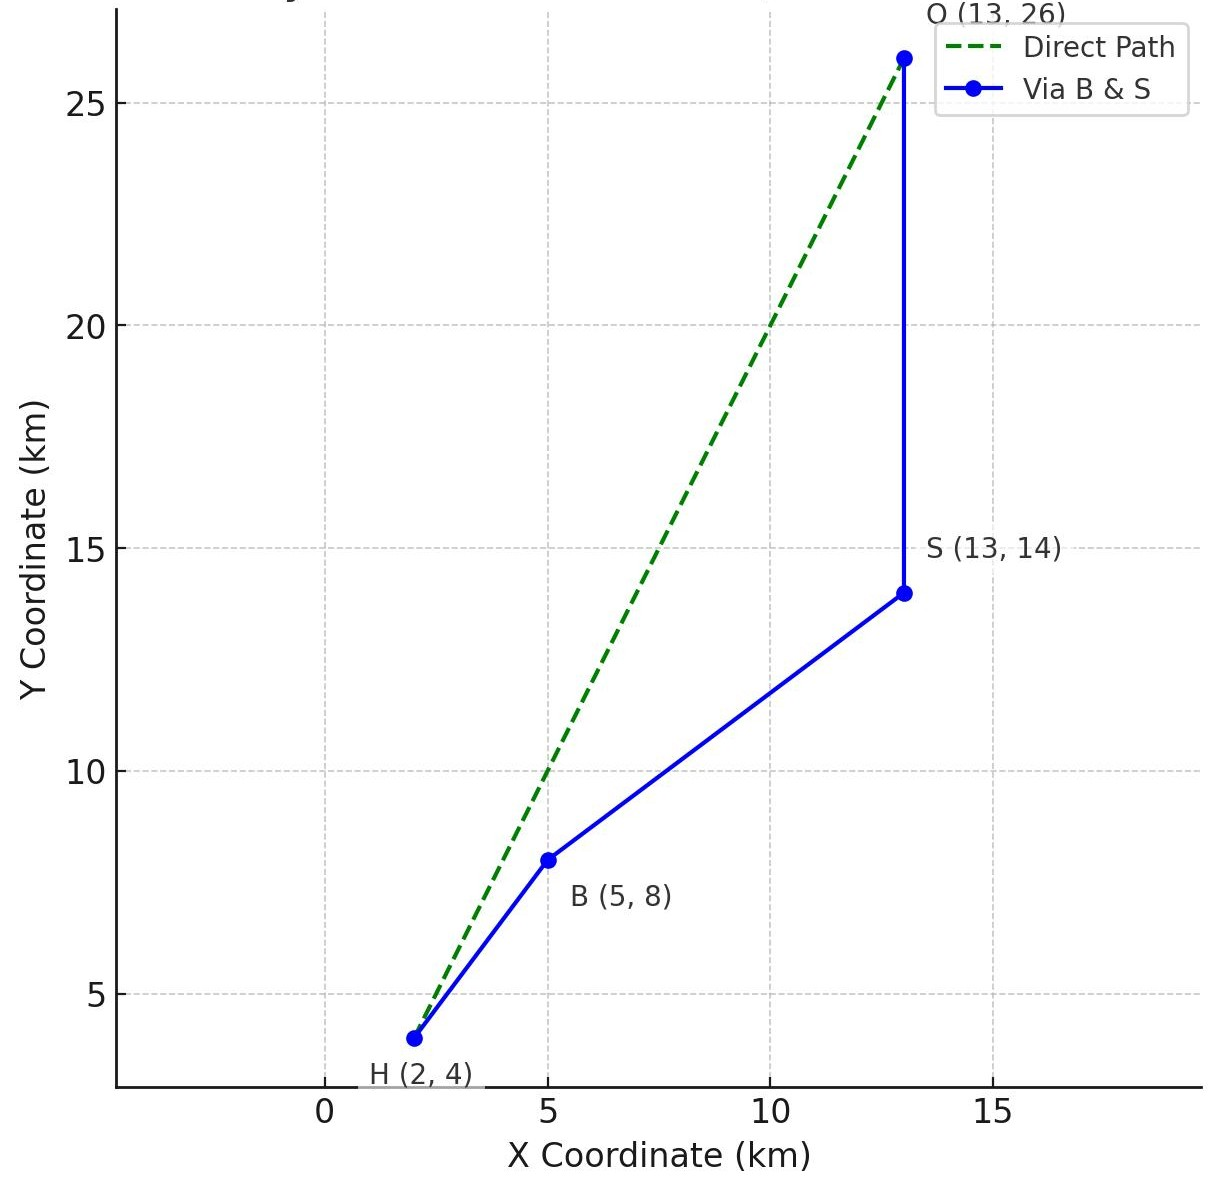
\includegraphics[width=0.7\columnwidth]{figs/graph.png}
 \caption*{Ayush's path to Office}
\label{fig:graph.png}
\end{figure}
\end{document}